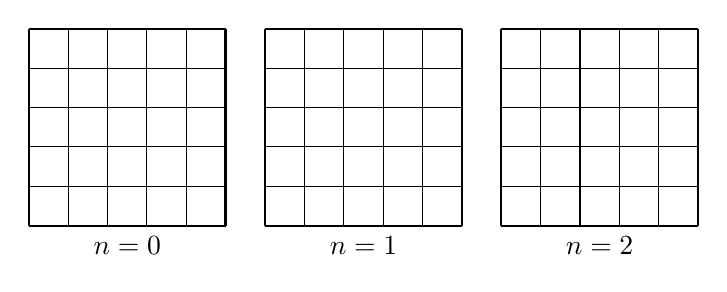
\begin{tikzpicture}[scale=.5]
    \begin{scope}
        \draw (0,0) grid (5, 5);
        \draw[thick, scale=5] (0, 0) grid (1, 1);

        \fillcell{1}{2}{dying}
        \fillcell{2}{1}{alive}
        \fillcell{3}{1}{dying}

        \node[anchor=center] at (2.5,-0.5) {$n=0$};
    \end{scope}

    \begin{scope}[xshift=6cm]
        \draw (0,0) grid (5, 5);
        \draw[thick, scale=5] (0, 0) grid (1, 1);

        \fillcell{2}{1}{dying}
        \fillcell{2}{2}{stillborn}

        \node[anchor=center] at (2.5,-0.5) {$n=1$};
    \end{scope}

    \begin{scope}[xshift=12cm]
        \draw (0,0) grid (5, 5);
        \draw[thick, scale=5] (0, 0) grid (1, 1);

        \node[anchor=center] at (2.5,-0.5) {$n=2$};
    \end{scope}
\end{tikzpicture}
